% ════════════════════════════════════════════════════════════════════
% SECTION 6 — RESULTS AND ANALYSIS  (v3.1: real frozen-protocol numbers)
% ════════════════════════════════════════════════════════════════════
\section{Results and Analysis}\label{sec:results}

All numbers in this section are produced by the improved pipeline
(improvements branch) under the frozen evaluation protocol of
Section~\ref{sec:experiments}: a single immutable
train/validation/test split, thresholds and calibration selected on
validation only, and the test set touched exactly once per model. Every
table and figure is generated from the machine-readable
results-json artefacts of the runs; no value is transcribed by
hand. The headline run uses 50 communication rounds, six clients, and
seed 42; Sections~\ref{sec:res-multiseed} and~\ref{sec:res-ablation}
quantify seed sensitivity and component attribution. An independent
re-execution of the headline pipeline from the public, byte-verified
dataset artefacts reproduces every test metric of every model exactly
(Section~\ref{sec:repro}); the calibration, frozen-FPR, and
client-holdout results below were produced in that re-execution
session.

\textbf{Protocol disclosure.} The data-provenance audit of
Section~\ref{sec:provenance} established that the in-partition
train/test pairing used by the shipped headline protocol shares
instances between the training pool and the test set---including
100\% of the flaring test instances. The subsections that follow the
present one therefore report \emph{in-partition} results: they remain
valid as evidence of protocol stability, seed sensitivity, component
attribution, and calibration behaviour under the frozen pipeline, but
they are not estimates of generalisation to unseen data. The
leakage-free evaluation under the benchmark's intended
temporally-preceding protocol is reported first, and the claims of
this study are tiered against it in
Section~\ref{sec:res-leakfree-discussion}.

\subsection{Leakage-free evaluation on the temporally-preceding fold}
\label{sec:res-leakfree}

Table~\ref{tab:leakfree} compares the five headline arms under the
leakage-free fold (training partitions 1--4, single-pass test on
partition 5) against the shipped in-partition numbers. Three
observations follow. First, \emph{discrimination generalises}: every
arm attains a ROC-AUC of at least 0.906 on the unseen partition, and
the task is evidently easier than the in-partition protocol suggested
(logistic regression reaches 0.978 / PR-AUC 0.455, the best PR ranking
of all arms together with XGBoost's 0.457). Second, the
centralised-versus-federated gap of the in-partition protocol
\emph{disappears}: the pooled centralised MLP of identical architecture
reaches 0.973 / 0.382 against FedProx's 0.976 / 0.308---a ROC
difference of 0.003 and a reversed PR ordering. The in-partition gap
(0.888 vs 0.954) was an artifact of the protocol pairing, not a
federation effect; the budget-parity re-run of
Section~\ref{sec:budget}, which controls optimisation budget but not
instance overlap, must be read in the same light. Third, the
FedProx-versus-FedAvg contrast partially survives: FedProx's ROC-AUC
(0.976) exceeds FedAvg's (0.906) by 0.070, but FedAvg's PR-AUC (0.370)
is \emph{higher} than FedProx's (0.308). The nuance is in the
checkpoint dynamics: plain FedAvg's validation F1 collapsed to zero by
round 40 and the protocol restored its round-35 checkpoint (validation
F1 0.915), so its leakage-free outcome depends on which round the
validation monitor happened to freeze. We no longer describe either
arm's outcome as checkpoint-independent: the BatchNorm diagnostic of
Section~\ref{sec:res-bn} shows the validation F1 monitor saturates at
the all-positive value $2p/(1+p)$ whenever the evaluated probabilities
saturate, and the checkpoint rule then acts on a saturated
signal---FedProx's apparent safety on this fold is that its evaluated
probabilities never crossed that regime, not that its artefact is
selection-invariant.

\begin{table}[t]
\centering
\caption{Leakage-free fold (train partitions 1--4, single-pass test on
partition 5, natural 1.31\% prevalence) against the shipped
in-partition numbers. Threshold-conditional calibration metrics
(Brier, ECE) use the validation-frozen prior-shift pipeline; ROC/PR
are threshold-free.}
\label{tab:leakfree}
\small
\begin{tabular}{@{}l c c c c c c c@{}}
\toprule
 & \multicolumn{2}{c}{\textbf{In-partition (shipped)}} &
 \multicolumn{5}{c}{\textbf{Leakage-free fold}} \\
\cmidrule(r){2-3} \cmidrule(l){4-8}
\textbf{Model} & ROC & PR & ROC & PR & Brier & ECE & R@2\%FPR \\
\midrule
Logistic regression & 0.824 & 0.235 & 0.978 & 0.455 & 0.375 & 0.477 & 0.695 \\
XGBoost (centralised) & 0.977 & 0.493 & 0.971 & 0.457 & 0.055 & 0.101 & 0.692 \\
Centralised MLP & 0.888 & 0.153 & 0.973 & 0.382 & 0.544 & 0.687 & 0.555 \\
FedAvg MLP & 0.575 & 0.199 & 0.906 & 0.370 & 0.127 & 0.337 & 0.652 \\
FedProx MLP & 0.954 & 0.307 & 0.976 & 0.308 & 0.271 & 0.508 & 0.631 \\
\bottomrule
\end{tabular}
\end{table}

The calibration and threshold-transfer failures documented
in-partition (Section~\ref{sec:res-calib}) persist leakage-free ---
on this fold the balanced-validation carve ($48.9\%$ prevalence,
partitions 1--4) again faces the natural-prevalence partition-5 test
($1.31\%$), the same 26-fold prior shift without the instance overlap ---
and are therefore genuine properties of the balanced-training /
natural-test interface rather than overlap artifacts: the
validation-frozen FPR operating points are violated by every arm
(e.g.\ XGBoost realises 15.3\% FPR at the frozen 2\% target; FedProx
49.4\%), and only XGBoost's posteriors remain usable (Brier 0.055,
ECE 0.101 versus 0.127--0.544 for the neural arms; FedAvg's 0.127
sits closest but is still an order of magnitude above the 0.013
climatology floor). The
prior-shift-corrected neural posteriors are not repairable by
threshold re-freezing on this fold either.

\paragraph{Standard verification metrics and baselines.}
Because the toolkit of Leka et al.~\cite{leka2019}---TSS, HSS, Brier
skill, reliability, persistence and climatology---is the standard
vocabulary of flare-forecast evaluation, it accompanies every stored
operating point of every evaluation substrate (the $F_\beta$
thresholds and frozen-FPR points of the in-partition, leakage-free
and raw-substrate 2-D arms, the ten raw-substrate LSTM cells, and
the event-level tables; 10-bin reliability is recomputed for the six
in-partition arms from the phase-cache models;
\texttt{experiments/run\_standard\_metrics.py} $\to$
\texttt{outputs/standard\_metrics.json}, strict JSON; the
artefact-derived blocks (A, C, D) are content-exact on re-execution,
block B's reliability recomputation additionally requires the
uncommitted phase-cache models, and the artefact embeds a wall-clock
\texttt{elapsed\_s} field, so file-level equality is not claimed).
Four findings matter. First, on the leakage-free fold
at each arm's frozen $F_\beta$ threshold, XGBoost attains TSS
$0.848$ / HSS $0.201$ (best frozen-FPR point $0.847$), logistic
regression TSS $0.489$ / HSS $0.025$, while the
neural arms sit at TSS $0.06$--$0.19$ / HSS $\le 0.006$: the
prevalence-free TSS ranking matches the PR-AUC ranking at the top
of the table (XGBoost, logistic regression, then the neural arms),
but HSS
prices the neural arms' false-alarm load severely at 1.31\%
prevalence. Second, the persistence baselines---computed on the true
time order within each active region, as the operational
verification culture mandates---set two floors, and neither is
decorative. Same-region previous-window persistence (label inertia)
achieves TSS $0.967$ / HSS $0.970$ on the partition-5 test with no
learned model at all: at a 24-hour label horizon on $\sim$60-minute
windows, an active region that is flaring is still flaring, and
\emph{no arm in this paper---XGBoost included---beats that floor}.
The 24-hour-lagged variant (forecast = the label of the same-region
window nearest $t-24$\,h, matched within $\pm$35 minutes) scores TSS
$0.418$ / HSS $0.434$; on TSS, XGBoost ($0.848$) and logistic
regression ($0.489$) are the only arms above it, and every
neural arm at its frozen threshold sits below it, while on HSS no
arm clears the floor at all (XGBoost's HSS is $0.201$). This is the
classic Leka-era result, and a benchmark audit is the right vehicle
for stating it plainly: at this window geometry the honest question
is not whether models beat persistence, but whether anything beats
\emph{lagged} persistence---and on this fold, at TSS, two arms do,
none at HSS. (An
earlier implementation of this baseline ordered windows by pool row,
whose within-region order is temporally scrambled---the median gap
between pool-row-adjacent windows is two days---so its stored value
measured randomly paired windows; that is precisely the class of
evaluation-protocol defect this paper exists to audit, and the
corrected ordering and both variants regenerate from the committed
artefact. A sensitivity sweep over eight candidate lag definitions
is committed alongside it
(\texttt{experiments/run\_lag\_definition\_sweep.py} $\to$
\texttt{outputs/lag\_definition\_sweep.json}): the seven point-lag
variants land at TSS $0.392$--$0.418$ with the same two arms
clearing each and none at HSS, while a lookback-flare variant
scores $0.964$---label inertia under another name, which no arm
clears---so the paper reports inertia and lagged persistence as
two distinct floors.) Third, no arm's raw Brier beats the climatology floor
(pooled-test BSS: XGBoost $-2.4$, FedAvg $-6.3$, FedProx $-13.3$;
all negative), and the 10-bin reliability tables confirm the
systematic over-confidence that the calibration analysis of
Section~\ref{sec:res-calib} dissects. Fourth, event-level detection
rates carry Wilson 95\% half-widths of $\pm$2.8--4.0 points on the
leakage-free fold and up to $\pm$11.8 points on the raw substrate
(65 events), and alert rates carry exact chi-square (Garwood)
Poisson intervals, so the between-arm event-level narrations of the
next paragraph are read against those bands.

\paragraph{Event-level evaluation.}
Table~\ref{tab:eventlevel} regroups the partition-5 test decisions
into physical flare events using the raw-benchmark event keys (65
M/X-class events; background windows grouped by region and day;
1-hour alert cooldown). All five arms detect effectively every event
(64--65 of 65) with a median first-alert lead time of 23.4\,h before
flare peak. That lead must be read for what it is: the label is
positive for \emph{every} window in the 24 hours before a flare, so a
median first alert near the horizon's edge measures the label
boundary, not precursor physics --- an honest reading is ``detection
fires early in the labelled window,'' not ``the model sees the flare
23 hours ahead.'' What separates the arms is their false-alarm
burden: XGBoost emits 1.7
false-alarm windows per day versus 11.6--12.7 for the neural arms, a
7$\times$ difference that mirrors the window-level calibration gap
and confirms that the deployability boundary on this benchmark is
calibration, not detection. After the 1-hour cooldown, roughly 70\%
of retained alerts are within-event duplicates, quantifying the
persistence behaviour an operations desk would face.

\begin{table}[t]
\centering
\caption{Event-level metrics on the leakage-free fold (65 true
M/X-class events, validation-frozen $F_2$ thresholds, 1-hour alert
cooldown). FA = false alarm.}
\label{tab:eventlevel}
\small
\begin{tabular}{@{}l c c c c@{}}
\toprule
\textbf{Model} & \textbf{Events detected} & \textbf{FA windows/day} &
\textbf{Alerts/day} & \textbf{Lead to peak (h)} \\
\midrule
Logistic regression & 65/65 (100\%) & 8.6 & 8.8 & 23.4 \\
XGBoost (centralised) & 64/65 (98.5\%) & 1.7 & 1.9 & 23.3 \\
Centralised MLP & 65/65 (100\%) & 12.7 & 12.8 & 23.4 \\
FedAvg MLP & 65/65 (100\%) & 11.6 & 11.8 & 23.4 \\
FedProx MLP & 65/65 (100\%) & 11.9 & 12.1 & 23.4 \\
\bottomrule
\end{tabular}
\end{table}

\subsection{Raw-substrate retraining: the unbalanced benchmark}
\label{sec:res-raw}

The leakage-free fold of Section~\ref{sec:res-leakfree} still trains
on the cleaned export---RUS--Tomek rebalanced, TimeGAN-augmented,
pre-normalised. The raw-benchmark retraining (re-run item~9,
executed in this revision) asks the complementary question: does anything in
the comparison survive when the frozen protocol is trained directly
on the \emph{raw} SWAN-SF partitions at their natural class
prevalence (2.05\% across training partitions 1--4), with no
rebalancing, no synthetic positives, and the two cleaning stages
reproduced in-pipeline? The raw benchmark cannot be trained on
directly: 8.87\% of its values are missing (42.3M of 476.9M; TOTFZ
is unobserved in 98.7\% of training windows) and the 24 parameters
span 11 orders of magnitude. The experiment therefore reproduces the
release's two preprocessing stages from their published description
(ApJS, 10.3847/1538-4365/ad7c4a): a \emph{fast
Pearson-correlation-based k-NN imputation} (partial gaps filled by
within-window interpolation; fully-missing series transferred from
the $k{=}5$ nearest training windows in the space of the five most
correlated observable features) and the \emph{LSBZM} normalisation
chain (robust clip, shift, log/sqrt/Box--Cox dispatched by fitted
$\lambda$, z-score, min--max), with every parameter fitted on the
training pool only. A verification against the released cleaned
export on the audit-matched partition-5 windows (100\% window match)
bounds the reproduction: at positions where the raw value was
observed and nonzero, rank agreement with the release has median
Spearman $\rho=0.898$ (min 0.842; the release is itself an exact
monotone image of the raw values, $\rho=1.000$, so the residual gap
is float16-storage tie dilution); at positions the release imputed,
agreement is method-dependent (median $\rho=0.313$), and for the
R-value flux-emergence proxy the release re-imputes the entire
zero mass (60.9\% of that column) as if it were missing, whereas
this reproduction preserves zeros as physical values. The three
substrates therefore differ in composition as well as in
preprocessing provenance, which is precisely the contrast the
experiment isolates.

Table~\ref{tab:rawsubstr} reports the six arms under the identical
frozen protocol (Dirichlet $\alpha{=}1.0$, six clients, 50 rounds,
Fed-Focal, seed 42, prior-shift calibration, validation-frozen
thresholds). The result is decisive and asymmetric.
\emph{Centralised arms are substrate-robust}: logistic regression is
unchanged to the third decimal (0.978, PR 0.448 vs 0.455), the
centralised MLP retains 0.971 ROC-AUC and its PR-AUC \emph{rises}
from 0.382 to 0.445, and XGBoost keeps 0.974 ROC-AUC while its
PR-AUC falls from 0.457 to 0.329---the synthetic TimeGAN positives
were inflating its minority-class precision, not teaching it.
\emph{Federated arms are substrate-fragile}: FedProx degrades from
0.976/0.308 to 0.930/0.149; plain FedAvg's PR-AUC collapses from
0.370 to 0.056 (its calibrated posteriors never cross the
validation-frozen threshold: test recall 0.000); and SCAFFOLD---the
one re-run item that had never been executed on any real
substrate---fails outright at 0.768/0.057 with Brier 0.137 (every
SCAFFOLD cell in this section measures the implementation's five
disclosed departures from the reference algorithm,
Section~\ref{sec:method}, and is read below as implementation-case
evidence). The
federated-versus-centralised ordering of the leakage-free fold was
still a property of the balanced training substrate; on the raw
unbalanced benchmark the focal-loss clients cannot learn the 2\%
minority class through 6-client Dirichlet heterogeneity, and the
gap between the best federated and best centralised arm widens to
0.048 ROC-AUC and $3\times$ PR-AUC.

One disclosure this section carried from v4.8, now resolved: the
three federated \emph{MLP} rows of Table~\ref{tab:rawsubstr} are
evaluated through the same untransported-BatchNorm path that
Section~\ref{sec:res-bn} indicts in-partition --- the runner
transports model \emph{parameters} only, so the returned
checkpoints carry never-updated running buffers into a
\texttt{model.eval()} evaluation. Until v4.9 the raw-substrate MLP
degradation above was therefore \emph{BN-evaluation-conditional} on
its face; the checkpoint-level diagnostic has since been executed
(Section~\ref{sec:res-rawbn}, \texttt{raw\_bn\_diagnostic.json}) and
the condition resolves \emph{against} the BN explanation: no
treatment recovers the centralised reference, pooled recalibration
actively destroys ranking, and the deficit is a property of the
flattened-feature arms under federation. The sequence arms are
outside the confound entirely (SolarLSTM carries no BatchNorm), so
the encoder-contrast reading of Section~\ref{sec:res-lstm} stands
either way.

\begin{table}[t]
\centering
\caption{Raw-substrate retraining (train raw partitions 1--4,
natural 2.05\% prevalence, FPCKNN/LSBZM reproduced in-pipeline with
train-only parameters; single-pass test on raw partition 5, natural
1.31\% prevalence; identical frozen protocol). The leakage-free
cleaned-substrate fold is reproduced for comparison; SCAFFOLD was
not run on the cleaned fold.}
\label{tab:rawsubstr}
\small
\begin{tabular}{@{}l c c c c c c@{}}
\toprule
 & \multicolumn{2}{c}{\textbf{Fold (cleaned)}} &
 \multicolumn{4}{c}{\textbf{Raw substrate}} \\
\cmidrule(r){2-3} \cmidrule(l){4-7}
\textbf{Model} & ROC & PR & ROC & PR & Brier & R@2\%FPR \\
\midrule
Logistic regression & 0.978 & 0.455 & 0.978 & 0.448 & 0.053 & 0.732 \\
XGBoost (centralised) & 0.971 & 0.457 & 0.974 & 0.329 & 0.018 & 0.587 \\
Centralised MLP & 0.973 & 0.382 & 0.971 & 0.445 & 0.010 & 0.596 \\
FedAvg MLP & 0.906 & 0.370 & 0.875 & 0.056 & 0.013 & 0.063 \\
FedProx MLP & 0.976 & 0.308 & 0.930 & 0.149 & 0.032 & 0.343 \\
SCAFFOLD MLP & --- & --- & 0.768 & 0.057 & 0.137 & 0.175 \\
\bottomrule
\end{tabular}
\end{table}

The event-level evaluation on the same substrate
(Table~\ref{tab:eventlevel-raw}) makes the collapse operational: all
65 true M/X-class events are matched to their GOES peaks exactly as
in the cleaned fold, but plain FedAvg now detects \emph{zero} of
them, FedProx detects 48 (73.8\%) at 1.3 false-alarm windows per
day, and SCAFFOLD's 83.1\% detection rate is bought at 6.4
false-alarm windows per day---roughly $20\times$ the centralised
arms' burden. The centralised arms detect 61.5--80\% of events at
0.2--0.3 false-alarm windows per day with 18--23\,h median lead
times. The sequence arms appended below the rule
(Section~\ref{sec:res-lstm}) restore partial federated detection
and are discussed there. Detection under class balance, in other
words, was the
artifact; under the benchmark's natural prevalence the deployable
models are exactly the ones that never needed federation.

\begin{table}[t]
\centering
\caption{Event-level metrics on the raw substrate (65 true M/X-class
events, validation-frozen $F_2$ thresholds, 1-hour alert cooldown;
99.86\% of test windows matched to the audit's event keys). The
sequence arms (below the rule) are evaluated by the standalone
torch-free CPU runner over the owner-GPU run's stored per-window
test probabilities and the same audit metadata; the SCAFFOLD-LSTM row
was evaluated in-runner by the same event-level machinery during
the second GPU batch. Median leads are rounded to 0.1\,h except the
SCAFFOLD-MLP cell, whose stored median (1{,}395\,min) is exactly
23.25\,h and is shown at full precision (T2 erratum, v4.8).}
\label{tab:eventlevel-raw}
\small
\begin{tabular}{@{}l c c c c@{}}
\toprule
\textbf{Model} & \textbf{Events detected} & \textbf{FA windows/day} &
\textbf{Alerts/day} & \textbf{Lead to peak (h)} \\
\midrule
Logistic regression & 51/65 (78.5\%) & 0.3 & 0.4 & 22.8 \\
XGBoost (centralised) & 40/65 (61.5\%) & 0.2 & 0.3 & 18.0 \\
Centralised MLP & 52/65 (80.0\%) & 0.3 & 0.4 & 20.5 \\
FedAvg MLP & 0/65 (0.0\%) & 0.0 & 0.0 & --- \\
FedProx MLP & 48/65 (73.8\%) & 1.3 & 1.4 & 23.0 \\
SCAFFOLD MLP & 54/65 (83.1\%) & 6.4 & 6.6 & 23.25 \\
\midrule
Centralised LSTM & 41/65 (63.1\%) & 0.3 & 0.4 & 19.3 \\
FedAvg LSTM & 35/65 (53.8\%) & 0.2 & 0.2 & 17.4 \\
FedProx LSTM & 49/65 (75.4\%) & 0.4 & 0.5 & 23.2 \\
SCAFFOLD LSTM & 55/65 (84.6\%) & 0.4 & 0.5 & 23.2 \\
\bottomrule
\end{tabular}
\end{table}

\subsection{Raw-substrate BN diagnostic: resolving the v4.8 condition}
\label{sec:res-rawbn}

The v4.8 revision shipped the runner for this diagnostic
(\texttt{experiments/run\_raw\_bn\_diagnostic.py}) and queued its
execution owner-side; it has since run (RUNLOG ask \#4), and its
artefact of record --- \texttt{outputs/raw\_bn\_diagnostic.json},
sha-pinned by the battery --- is what this subsection reads. One
structural fact precedes the numbers, disclosed at equal length in the
RUNLOG: the v3.x-era raw-substrate checkpoints were \emph{never
persisted} (that era's runner stored the 3D caches and the
sequence-arm checkpoints, not the seed-42 MLP weights), so the
same-weights counterfactual the diagnostic was designed around is
unavailable by construction. The run therefore re-evaluated a fresh
seed-42 replication: the substrate was rebuilt from the surviving 3D
cache (one additional f16 quantisation, within the $5\times10^{-3}$
series bound the cache format documents), the three arms were
retrained round-resumably under the frozen protocol, and the
diagnostic then applied its three BN treatments to those identical
weights. The replication is close at the substrate level: the pooled
baselines reproduce the published rows to $\le 2.3\times10^{-3}$
ROC-AUC (logistic regression $+1.7\times10^{-4}$, XGBoost
$+1.5\times10^{-3}$, centralised MLP $-2.3\times10^{-3}$), which
isolates the federated arms' gate deltas --- ROC-AUC $+0.023$
(FedAvg), $-0.002$ (FedProx), $-0.005$ (SCAFFOLD) --- as retrain
nondeterminism concentrated in the highest-variance arm. The gate
recorded MISMATCH on all three arms (tolerance $10^{-4}$) and exited
non-zero as designed; the record is frozen with that verdict.

\begin{table}[t]
\centering
\caption{The raw-substrate BN diagnostic
(\texttt{raw\_bn\_diagnostic.json}, v4.9): test ROC-AUC / PR-AUC of
the identical replication weights under the three BN treatments, per
federated MLP arm. A: the published init-buffer evaluation path; B:
exact per-client statistics pooled by the law of total variance
(training shards only); C: evaluation-time batch statistics. Gate
$\Delta$ is arm A's ROC-AUC delta against the published rows of
Table~\ref{tab:rawsubstr} (the disclosed MISMATCH; FedAvg carries
the replication's retrain variance).}
\label{tab:rawbndiag}
\small
\begin{tabular}{@{}l c c c c@{}}
\toprule
\textbf{Arm} & \textbf{A: init buffers} & \textbf{B: pooled} &
\textbf{C: batch stats} & \textbf{Gate $\Delta$} \\
\midrule
FedAvg   & 0.898 / 0.070 & 0.501 / 0.015 & 0.915 / 0.227 & $+0.023$ \\
FedProx  & 0.928 / 0.149 & 0.500 / 0.013 & 0.920 / 0.251 & $-0.002$ \\
SCAFFOLD & 0.763 / 0.053 & 0.500 / 0.013 & 0.757 / 0.069 & $-0.005$ \\
\bottomrule
\end{tabular}
\end{table}

Table~\ref{tab:rawbndiag} yields the reading, and it is the opposite
of the in-partition pattern of Section~\ref{sec:res-bn}. First,
\emph{the raw-substrate MLP deficit is not a manufactured collapse}:
arm A --- the very path the in-partition diagnostic indicts --- holds
0.763--0.928 ROC-AUC on every arm here, where the in-partition
collapse scored 0.575, and no treatment approaches the centralised
reference (0.969 on the same replication): the residual deficit,
roughly 0.04--0.21 ROC-AUC depending on arm and treatment, is a
property of the flattened-feature arms under federation, not of the
buffer-transport protocol. Second, \emph{pooled recalibration is
actively destructive here}: arm B collapses every arm to chance
(0.500--0.501), whereas in-partition the same oracle \emph{recovered}
FedAvg from 0.575 to 0.893 --- pooling exact per-client statistics
across 6 heterogeneous raw-prevalence clients inflates variance past
the point where any single pooled normalisation ranks the test
distribution, so the in-partition ``optimistic recalibration rescue''
does not transfer to the natural-prevalence substrate at all. Third,
evaluation-time batch statistics (arm C) move ROC-AUC by at most
0.017 while sharpening the positive score scale (PR-AUC
0.070$\to$0.227 for FedAvg, 0.149$\to$0.251 for FedProx): a
calibration instrument, not a rescue. The diagnostic's event-level
layer also records the operating-point pathology the A-path
thresholds inherit --- the replication's checkpoint rule returned
best-val-F1 states of 0.0 for FedAvg and FedProx, FedAvg's val-frozen
threshold sat at the 0.05 floor, and the arm detects 0 of 65 events
under A while arm C, the only treatment with a usable validation
operating point, detects 38 (58.5\%) at 0.28 false-alarm windows per
day (FedProx: 62 at 2.8 under A, 50 at 0.43 under C). The v4.8
condition is therefore closed with a precise scope: untransported BN
statistics can manufacture collapse --- in-partition proved that ---
but the raw-substrate federated MLP degradation is not that
phenomenon, and the sequence arms (no BatchNorm) were never exposed
to it.

\subsection{The sequence encoder rescues the federated arms}
\label{sec:res-lstm}

The raw-substrate collapse of Table~\ref{tab:rawsubstr} is a
statement about the flattened-feature MLP arms, and the second half of
re-run item~8 asks exactly that question: does the same frozen
protocol survive natural prevalence when the federated encoder is
sequential? The LSTM arms were executed on owner-side GPU hardware
(RTX\,4060 Laptop, cuDNN; 2.6\,h total wall-clock for both
federated arms plus the pooled comparator, against a CPU-only
sandbox run that would have been impractically slow---the one experiment where a GPU was a
practical requirement rather than a convenience). The
substrate is identical by construction: the runner rebuilds the 3D
series from the same cached stage-A/B arrays, asserts label equality
with the frozen 2D split at startup, runs the 144-statistic feature
cross-check whenever the 2D cache is present (max$|$diff$|$ bounded
by $5\times10^{-3}$ at float16 storage; on the owner-GPU box the
label-equality assertion alone ran, the 2D cache being absent
there), and reuses the
identical seed-42 Dirichlet shards, so the only degrees of freedom
are the encoder and the device. The SolarLSTM (219,265 parameters,
consuming the raw $60\times24$ series directly) is trained under the
same Fed-Focal loss, prior-shift calibration, and validation-frozen
threshold machinery as every other arm. The one arm still unexecuted
in the second owner-GPU batch---SCAFFOLD-LSTM, whose MLP instance is the hardest failure
on this substrate---was subsequently run in a second owner-GPU batch
together with the seed-43 replication and the SMOTE ablation
reported below, under the client-side fixed-step SGD that the
control-variate arithmetic requires (the AdamW invalidation of
Section~\ref{sec:discussion} is avoided by construction in the
federated implementation).

Table~\ref{tab:lstmraw} reports the outcome alongside each arm's
frozen MLP counterpart, and the asymmetry of
Section~\ref{sec:res-raw} inverts. Centrally, the LSTM is the
\emph{weaker} architecture: 0.962/0.314 against the central MLP's
0.971/0.445 on the same windows. Federated, the ordering reverses.
FedAvg-LSTM holds 0.958/0.305 where the FedAvg MLP fell to
0.875/0.056---a $+0.083$ ROC-AUC and $+0.249$ PR-AUC swing from the
encoder alone, under identical shards, budgets, and aggregation.
FedProx-LSTM reaches 0.970/0.404: above its own pooled centralised
comparator ($+0.008$ ROC, $+0.090$ PR) and above XGBoost's raw
PR-AUC (0.329). SCAFFOLD-LSTM lands at 0.970/0.294 against its MLP
counterpart's 0.768/0.057---the largest single encoder swing on
this substrate ($+0.202$ ROC-AUC, $+0.238$ PR-AUC): the hardest
failure of the flattened-feature matrix is fully recovered by the
sequence encoder under the identical protocol, completing the
four-arm federation matrix on this benchmark. The two contrasts isolate what happened. Between
federated arms of identical budget and aggregation, the sequence
encoder removes the natural-prevalence collapse the MLP suffers; the
load-bearing comparison is budget-matched by construction. Between
the pooled and federated instances of the same sequence encoder,
federation costs nothing (FedAvg) or appears to help (FedProx)---but
the latter margin carries a budget caveat, since the central
comparator is capped at 30 epochs while the federated arms receive
500 shard passes, and the cleaned-fold parity experiment moved the
central MLP by $+0.029$ ROC-AUC under exactly that correction
(Section~\ref{sec:budget}).

What does not change is at least as important. No federated arm
exceeds the best centralised baseline on either rank metric
(FedProx-LSTM sits 0.008/0.044 below logistic regression). The
frozen-$F_\beta$ thresholds transfer badly for three of the four
arms: validation $F_2$ values of 0.727/0.765/0.593 degrade to test
values of 0.405/0.309/0.499 under the $1.6\times$ validation-to-test
prevalence shift, while SCAFFOLD-LSTM is the exception---its
validation $F_2$ of 0.530 lands at 0.528 on test at a recall-heavy
operating point (test recall 0.737)---and the frozen-FPR operating
points still realise their targets within band, reproducing
(including the same conservative drift at the 0.5\% target) the
behaviour already documented for the MLP arms. Calibration remains
the deployability boundary: all three federated sequence arms beat
the raw-substrate climatology floor of 0.013 (FedAvg 0.0112,
FedProx 0.0106, SCAFFOLD 0.0120, against every federated MLP arm at
or above it, 0.013--0.137), but FedProx-LSTM's ECE of 0.020 is four
times the central LSTM's 0.005, SCAFFOLD-LSTM carries the worst
sequence-encoder calibration (0.035), and the centralised MLP's
Brier of 0.010 remains the best of all ten arms executed on this
substrate. Finally, the FedProx-over-FedAvg stabilisation now
appears on every substrate--encoder combination executed
(in-partition MLP 0.954 vs 0.575; cleaned fold 0.976 vs 0.906; raw
MLP 0.930 vs 0.875; raw LSTM 0.970 vs
0.958, replicated at seed 43 as 0.965 vs 0.961)---the most
replicated single finding of this study. The
event-level pass (bottom block of Table~\ref{tab:eventlevel-raw})
was executed offline, on CPU, from the GPU run's stored per-window
test probabilities over the same audit metadata---no retraining,
65/65 GOES peaks matched. Where plain FedAvg-MLP detects \emph{zero}
of the 65 events, FedAvg-LSTM detects 35 (53.8\%) at 0.2
false-alarm windows per day: the encoder rescue survives the
validation-frozen thresholds and the cooldown machinery, not just
the ranking metrics. FedProx-LSTM is the standout: 49/65 (75.4\%)
detection at 0.4 false-alarm windows per day, exceeding
FedProx-MLP's raw detection while cutting its false-alarm burden
$3.5\times$ (1.3), with a 23.2\,h median first-alert lead to flare
peak---the joint-longest on this substrate, and (like every arm's
lead at this label geometry) a label-boundary quantity rather than a
usable warning time (Table~\ref{tab:eventlevel}). SCAFFOLD-LSTM---measuring,
like every SCAFFOLD cell, the sign-inverted, cold-start variant of
the five-departure list in Section~\ref{sec:method}, not the
reference algorithm---evaluated in-runner by the same machinery,
supplies the sharpest
event-level datum of the batch: 55/65 (84.6\%) detection at 0.41
false-alarm windows per day and a 23.2\,h median lead---its MLP
twin's 83.1\% detection rate at one-fifteenth its false-alarm
burden, and nominally above the centralised detection frontier
(logistic regression 78.5\%, centralised MLP 80.0\%, both at
0.2--0.3 per day). The crossing is an operating-point purchase
rather than a ranking win---it is bought with $1.5$--$2\times$ the
centralised arms' alarm budget, the window-level ranking still
sits below logistic regression by 0.008/0.154, and the arm carries
the worst sequence-encoder calibration (ECE 0.035)---so the
data-locality conclusion of Section~\ref{sec:res-raw} survives at
event level with this one priced exception.

\begin{table}[t]
\centering
\caption{Raw-substrate LSTM arms (frozen protocol, identical
substrate, shards, and evaluation as Table~\ref{tab:rawsubstr};
owner-GPU execution, seed 42) with each arm's frozen MLP counterpart
repeated from Table~\ref{tab:rawsubstr} for the
architecture-versus-federation contrast. Brier and ECE on the
calibrated test probabilities at natural 1.31\% prevalence. The
seed-43 replication and per-client SMOTE ablation of the same arms
are reported in Table~\ref{tab:lstmrep}.}
\label{tab:lstmraw}
\small
\begin{tabular}{@{}l cc cc c c c@{}}
\toprule
 & \multicolumn{2}{c}{\textbf{LSTM arm}} &
 \multicolumn{2}{c}{\textbf{MLP counterpart}} & & & \\
\cmidrule(r){2-3} \cmidrule(l){4-5}
\textbf{Model} & ROC & PR & ROC & PR & Brier & ECE & R@2\%FPR \\
\midrule
Centralised & 0.962 & 0.314 & 0.971 & 0.445 & 0.0111 & 0.005 & 0.481 \\
FedAvg & 0.958 & 0.305 & 0.875 & 0.056 & 0.0112 & 0.007 & 0.431 \\
FedProx & 0.970 & 0.404 & 0.930 & 0.149 & 0.0106 & 0.020 & 0.525 \\
SCAFFOLD & 0.970 & 0.294 & 0.768 & 0.057 & 0.0120 & 0.035 & 0.521 \\
\bottomrule
\end{tabular}
\end{table}

\subsection{Seed replication and the natural-prevalence SMOTE
ablation}
\label{sec:res-lstmrep}

The sequence arms executed at a single seed on a single
device, and the replication caveat that followed them is discharged
by the second owner-GPU batch: all four arms re-executed at seed 43
(model initialisation and the Dirichlet shard draw reseeded, the
frozen validation carve kept identical). The ranking structure
replicates (Table~\ref{tab:lstmrep}, middle columns)---the seed-42
FedProx/SCAFFOLD statistical tie (0.970 each) resolving into
SCAFFOLD's narrow lead at seed 43.
ROC-AUC moves by at most 0.005 on any arm (FedAvg
0.958$\to$0.961, FedProx 0.970$\to$0.965, SCAFFOLD
0.970$\to$0.968, central 0.962$\to$0.962)---inside the device and
kernel jitter band predicted in Section~\ref{sec:repro}---and
every qualitative finding survives: no arm collapses, FedProx
stays above FedAvg on both rank metrics, SCAFFOLD stays
competitive, and no federated arm approaches the centralised
ranking frontier. PR-AUC, as expected at 1.3\% prevalence, moves
more (FedAvg 0.305$\to$0.271, central 0.314$\to$0.357, SCAFFOLD
0.294$\to$0.368, FedProx 0.404$\to$0.381) without overturning any
load-bearing ordering. Event-level detection moves within a
seven-point band at comparable false-alarm rates (FedAvg
35$\to$36, central 41$\to$43, FedProx 49$\to$45, SCAFFOLD
55$\to$50 of 65). The sequence-encoder rescue is not an artefact
of one seed.

\begin{table}[t]
\centering
\caption{Seed-43 replication and per-client SMOTE ablation of the
raw-substrate sequence arms (window-level test metrics; protocol,
substrate, and evaluation identical to
Table~\ref{tab:lstmraw}). Seed 43 reseeds model initialisation and
the Dirichlet shard draw; the frozen validation carve is unchanged.
SMOTE oversamples each client's minority class to a 0.25
minority-to-majority ratio (seed 42, flattening the $60\times24$
series and reshaping).}
\label{tab:lstmrep}
\small
\begin{tabular}{@{}l cc cc cc@{}}
\toprule
 & \multicolumn{2}{c}{\textbf{Seed 42}} &
 \multicolumn{2}{c}{\textbf{Seed 43}} &
 \multicolumn{2}{c}{\textbf{Seed 42 + SMOTE}} \\
\cmidrule(r){2-3} \cmidrule(r){4-5} \cmidrule(l){6-7}
\textbf{Model} & ROC & PR & ROC & PR & ROC & PR \\
\midrule
Centralised & 0.962 & 0.314 & 0.962 & 0.357 & --- & --- \\
FedAvg & 0.958 & 0.305 & 0.961 & 0.271 & 0.961 & 0.307 \\
FedProx & 0.970 & 0.404 & 0.965 & 0.381 & 0.946 & 0.288 \\
SCAFFOLD & 0.970 & 0.294 & 0.968 & 0.368 & --- & --- \\
\bottomrule
\end{tabular}
\end{table}

The complementary ablation asks whether class rebalancing can
substitute for the encoder. Per-client SMOTE, oversampling each
shard's minority to a 0.25 minority-to-majority ratio on the
flattened $60\times24$ series, was run for the two production
federated arms at seed 42 (Table~\ref{tab:lstmrep}, right columns).
FedAvg is unchanged at window level (0.961/0.307 against 0.958/0.305
natural, with event detection even edging up, 35$\to$40 of 65);
FedProx is actively degraded:
0.946/0.288 against 0.970/0.404, a $-0.116$ PR-AUC loss, with
event detection falling 49$\to$37 of 65. The result completes the
cleaned-fold SMOTE null (Section~\ref{sec:res-ablation}: inert
there because the substrate was pre-balanced) at natural
prevalence, where it has work to do: oversampling is no substitute
for the encoder and costs the strongest arm 0.116 of its 0.404
PR-AUC. This is consistent with the loss-stacking analysis of
Section~\ref{sec:discussion}---SMOTE, the focal $\alpha$, and
class-rate-aware aggregation all adjust the same effective
positive-class weight, and stacking a second balancing mechanism on
the protocol's existing ones overshoots. The rescue is
architectural; class balance is neither necessary nor sufficient.

\subsection{What survives the leakage-free protocol}
\label{sec:res-leakfree-discussion}

With the raw-substrate retraining of Section~\ref{sec:res-raw} the
comparison now spans three substrates---in-partition (overlap
disclosed), leakage-free cleaned (rebalanced, synthetic positives),
and leakage-free raw (natural prevalence)---and the surviving claims
can be tiered across all three. Two claims transfer unchanged to
\emph{every} substrate: the \emph{deployability boundary} (only
XGBoost's posteriors survive the prevalence shift on the cleaned
fold; on the raw substrate the centralised MLP's Brier of 0.010
remains the best of all ten arms, with the three federated sequence
arms the only federated results to beat the climatology floor
(Brier 0.011--0.012 versus 0.013, FedProx-LSTM the best of them at
an ECE of 0.020 against the central arms'
0.005--0.011) and the \emph{threshold-transfer failure} at fixed-FPR
operating points. FedProx's \emph{ROC stabilisation} over plain FedAvg---a composite
of genuine early-round optimisation benefit and compatibility with the
shipped evaluation path (Sections~\ref{sec:res-bn}--\ref{sec:res-nobn})---transfers
to the cleaned fold (0.976 vs 0.906) and, in diminished form, to the
raw substrate (0.930 vs 0.875 for the MLP arms; 0.970 vs 0.958 for
the sequence arms of Section~\ref{sec:res-lstm}); it is the only
claim now observed on every substrate executed and on both encoders
wherever both were run. Three
claims do not transfer beyond the cleaned fold, and all three are
statements about the \emph{MLP} arms: the
federated-versus-centralised ROC gap (0.003 on the cleaned fold,
0.048 in favour of centralised on raw; 0.008 for the sequence arms),
FedProx's in-partition PR-AUC edge (its raw PR-AUC of 0.149 is a
third of the centralised MLP's 0.445, though the sequence arm
reaches 0.404), and the absolute discrimination levels of the
flattened-feature federated arms themselves (FedAvg-MLP detects zero
of 65 events on the raw substrate; the sequence arm detects 35,
Section~\ref{sec:res-lstm}).
The multi-seed, sweep, ablation, and client-level
studies of the following subsections were executed under the
in-partition protocol and are retained as protocol-stability
evidence; their leakage-free and raw-substrate counterparts remain
queued, though the sequence arms' seed replication is now discharged
(Section~\ref{sec:res-lstmrep}; fold-replication remains owner-side
compute).

\subsection{Headline comparison on the held-out test set (in-partition protocol)}

\begin{table}[t]
\centering
\caption{Single-pass test-set evaluation at natural prevalence
($n{=}331{,}185$, $1.88\%$ positives), at each model's
$F_2$-optimal threshold $\tau^\ast$ selected on \emph{validation}.
Calibration: prior-shift (fit on validation). Brier and ECE (15 bins)
are computed on the calibrated probabilities. Best value per column in
bold; the climatology row is the validation-fitted base rate (the
prior-shift convention), and the honest Brier reference is the
test-set climatology ($0.0185$ at 1.88\% prevalence), which no arm's
calibrated Brier beats---see Section~\ref{sec:res-calib}.}
\label{tab:main}
\footnotesize
\setlength{\tabcolsep}{2.8pt}
\begin{tabularx}{\textwidth}{@{}>{\raggedright\arraybackslash}X c c c c c c c c@{}}
\toprule
\textbf{Model} & $\boldsymbol{\tau^\ast}$ & \textbf{Prec.} &
\textbf{Recall} & \textbf{F1} & \textbf{ROC-AUC} & \textbf{PR-AUC} &
\textbf{Brier} & \textbf{ECE} \\
\midrule
Climatology & 0.05 & 0.019 & 1.000 & 0.037 & 0.500 & 0.019 & 0.239 & 0.470 \\
Logistic regression & 0.23 & 0.021 & 0.967 & 0.041 & 0.824 & 0.235 & 0.659 & 0.732 \\
Centralised MLP & 0.32 & 0.030 & 0.999 & 0.059 & 0.888 & 0.153 & 0.277 & 0.439 \\
XGBoost (centralised ref.) & 0.37 & \textbf{0.146} & 0.968 &
\textbf{0.254} & \textbf{0.977} & \textbf{0.493} & \textbf{0.063} &
\textbf{0.115} \\
FedAvg MLP (federated) & 0.36 & 0.020 & 0.997 & 0.038 & 0.575 & 0.199 & 0.136 & 0.342 \\
FedProx MLP (federated) & 0.51 & 0.021 & 0.999 & 0.042 & 0.954 & 0.307 & 0.264 & 0.496 \\
\bottomrule
\end{tabularx}
\end{table}

Table~\ref{tab:main} contains four findings. \textbf{(i)~The
architecture-controlled comparison now exists.} The v2.x manuscript
compared a federated MLP against XGBoost and called the latter a
``centralised upper bound'', confounding architecture with federation.
With the centralised MLP of the identical 29{,}377-parameter
architecture, the comparison isolates the effect of federation from
the effect of architecture---but \emph{not} from optimisation budget
(Section~\ref{sec:budget}: the federated arm consumed the larger
budget, 500 effective local passes versus at most 30 pooled passes).
Under that caveat, FedProx (ROC-AUC 0.954, PR-AUC 0.307) did not
underperform its pooled counterpart (0.888, 0.153) on this benchmark
and configuration---an observation consistent with non-IID federated
training plus a proximal regulariser acting as an implicit regulariser
for this small MLP, and which we do \emph{not} generalise to the claim
that federation is free of cost. \textbf{(ii)~The shipped evaluation separates FedAvg and FedProx,
but the separation is largely an evaluation-path property.} Plain
FedAvg's shipped trajectory drifts (Section~\ref{sec:res-conv}) and
its best-validation checkpoint reaches 0.575 ROC-AUC as evaluated;
Sections~\ref{sec:res-bn}--\ref{sec:res-nobn} show the same weights
carry 0.951 under correct normalisation and that neither algorithm
diverges without BatchNorm, so the proximal term is the difference
between compatibility and incompatibility with the shipped evaluation
path \emph{under the frozen-protocol configuration}, plus a modest
early-round optimisation benefit. \textbf{(iii)~Against the strongest
reference,} FedProx retains $97.7\%$ of XGBoost's ROC-AUC and $62\%$
of its PR-AUC. \textbf{(iv)~The $\tau^\ast$ column exposes a
protocol-honest failure}: thresholds optimised for $F_2$ at the
validation prevalence ($48.9\%$) transfer poorly to the $1.88\%$ test
prevalence---all neural models fire almost unconditionally (recall
$\approx 1.0$, precision $\approx$ the base rate), and the calibration
columns (Brier, ECE) show every neural model \emph{worse calibrated
than the climatology}. We analyse this threshold-transfer failure
explicitly in Section~\ref{sec:res-calib} and report prevalence-robust
operating points instead.

\subsection{Prevalence-robust discrimination: ROC and PR analysis}

\begin{figure}[t]
    \centering
    \begin{adjustbox}{max width=0.72\textwidth, max height=0.42\textheight}
        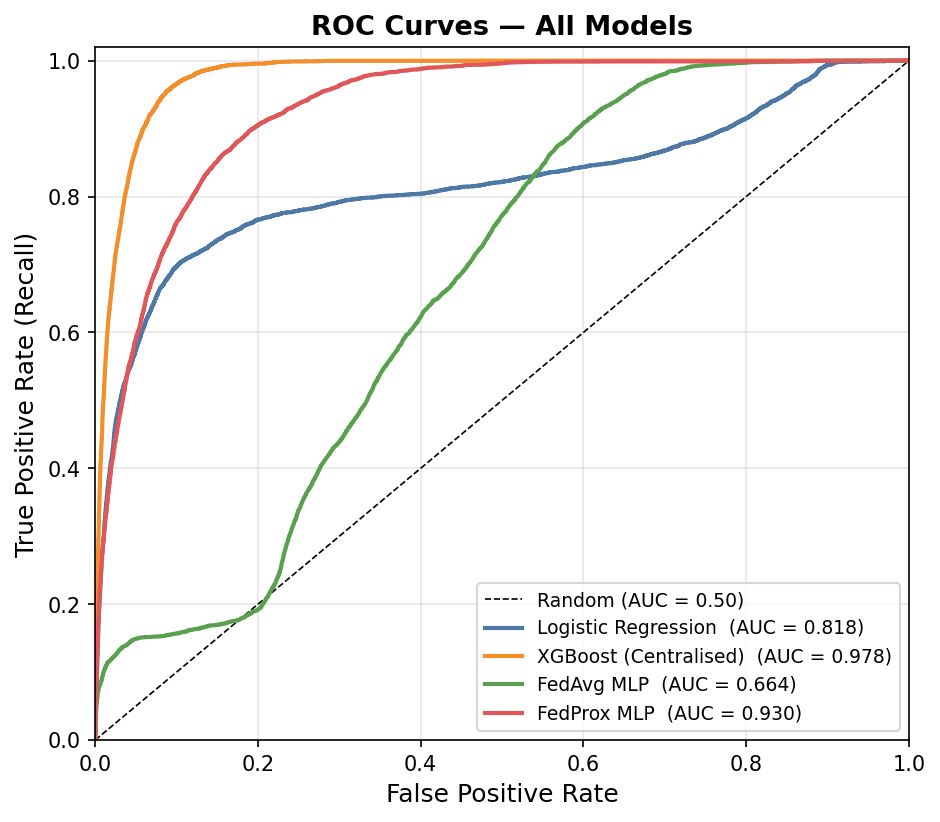
\includegraphics{figures/ROC_Curves.png}
    \end{adjustbox}
    \caption{ROC curves on the held-out test set. FedProx (AUC 0.954)
    tracks the centralised XGBoost reference (0.977) across the
    low-false-positive region; the centralised MLP (0.888) sits between
    them; FedAvg (0.575) evaluates far below its weights' actual
    information content (Section~\ref{sec:res-bn}: 0.951 under correct
    normalisation).}
    \label{fig:roc}
\end{figure}

Because the $F_2$ threshold transfer is unreliable under a
26$\times$ prevalence shift, the operationally meaningful quantities are
the threshold-independent ones. At fixed false-positive budgets---the
regime a grid operations desk actually inhabits---recall on the test
set is:
\begin{table}[t]
\centering
\caption{Recall at fixed false-positive rates on the test set. These
are \emph{discrimination curve statistics}: for each budget, the recall
at the point of the test ROC curve where FPR equals the target. They
involve no threshold transfer from validation and are therefore robust
to monotone miscalibration, but they are \emph{window-level}
quantities: the 60-minute sliding windows of one active region are
correlated, so a 2\% window-level FPR does not translate directly into
an operational false-alarm rate per event or per day (event-level
evaluation: Section~\ref{sec:limitations}).}
\label{tab:recallfpr}
\small
\begin{tabularx}{0.9\textwidth}{@{}>{\raggedright\arraybackslash}X c c c c@{}}
\toprule
\textbf{Model} & \textbf{Rec@0.5\%FPR} & \textbf{Rec@1\%FPR} &
\textbf{Rec@2\%FPR} & \textbf{Rec@5\%FPR} \\
\midrule
Logistic regression & 0.199 & 0.287 & 0.419 & 0.568 \\
Centralised MLP & 0.101 & 0.147 & 0.220 & 0.384 \\
XGBoost (centralised ref.) & \textbf{0.346} & \textbf{0.484} &
\textbf{0.651} & \textbf{0.864} \\
FedAvg MLP & 0.164 & 0.247 & 0.380 & 0.443 \\
FedProx MLP & 0.221 & 0.345 & 0.506 & 0.712 \\
\bottomrule
\end{tabularx}
\end{table}

Three readings matter. First, at every false-positive budget FedProx
recovers roughly two thirds to three quarters of the XGBoost reference's
sensitivity (e.g.\ $0.506$ vs $0.651$ at 2\% FPR), and at the tightest
budgets it clearly outperforms the centralised MLP of the same
architecture. Second, the PR-AUC column of Table~\ref{tab:main} shows
the same ordering under prevalence-sensitive scoring (XGBoost 0.493,
FedProx 0.307, FedAvg 0.199): in the high-precision region the federated
model pays a real ranking price relative to the ensemble, even though it
beats its own architecture's pooled baseline. Third, FedAvg's recall
profile decays fastest with tightening budget---\emph{as evaluated}.
Section~\ref{sec:res-bn} shows this to be a property of the evaluation
path, not of the weights: the same checkpoint holds 0.951 ROC-AUC of
ranking information under correct normalisation.

\subsection{Convergence behaviour: the evaluated drift and its suppression}
\label{sec:res-conv}

\begin{figure}[t]
    \centering
    \begin{adjustbox}{max width=0.96\textwidth, max height=0.34\textheight}
        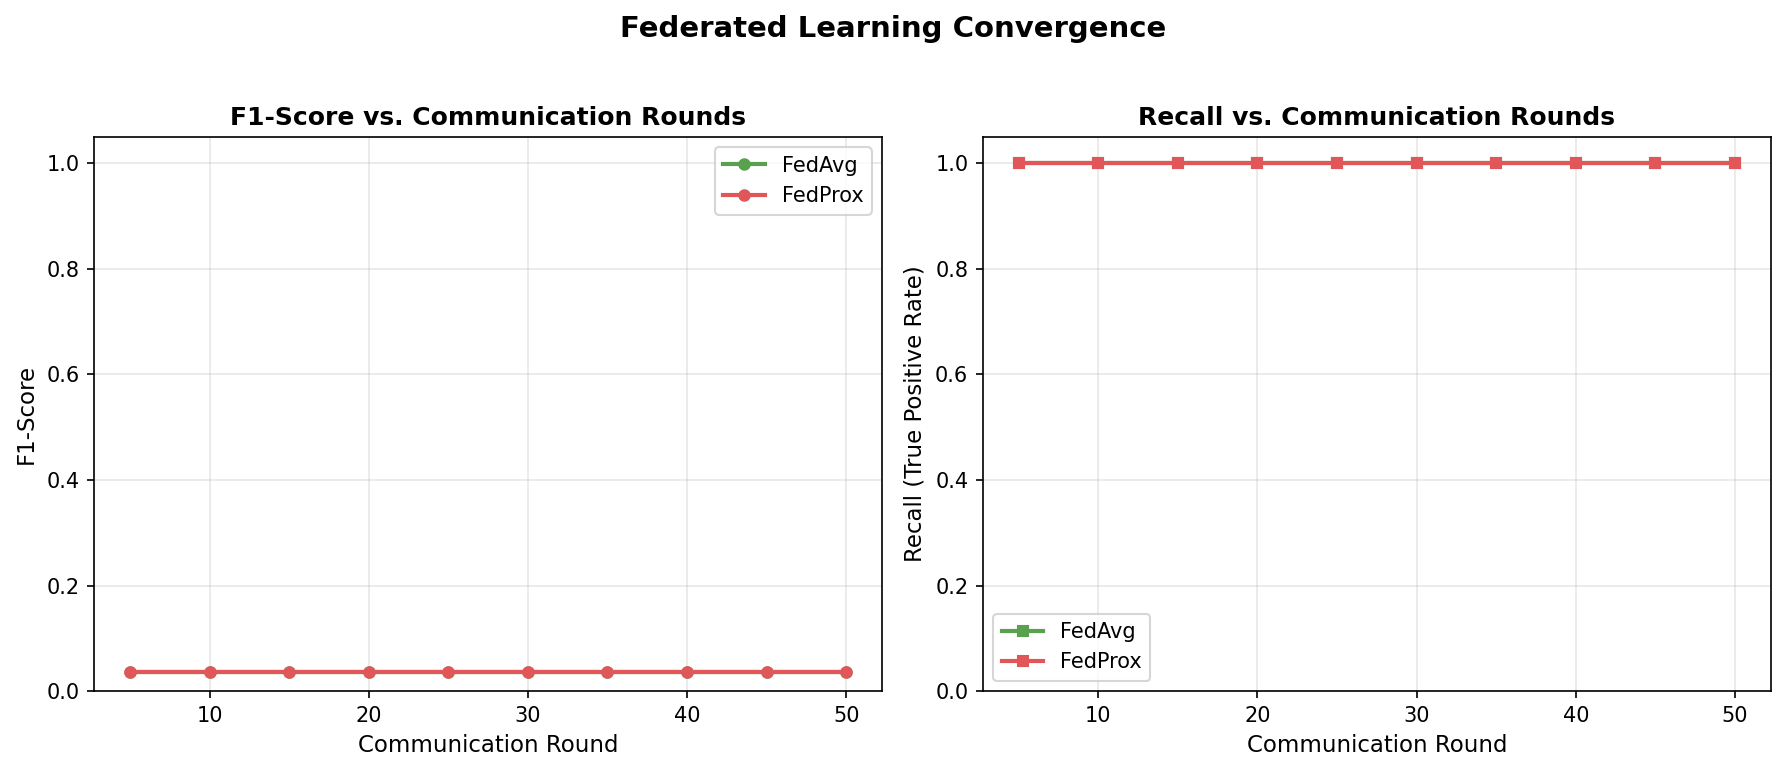
\includegraphics{figures/FL_Convergence.png}
    \end{adjustbox}
    \caption{Validation-monitored convergence over 50 rounds: per-round
    validation F1 (left panel) and validation Recall (right panel) at
    the development threshold, as evaluated by the shipped server-side
    path (FedAvg vs FedProx; ROC-AUC values quoted in the text come
    from the round-level validation history in the run artefacts, not
    from this figure). Plain FedAvg's evaluated F1 collapses toward
    zero after round 20 while its recall saturates at 1.0 (the
    all-positive degenerate regime); FedProx ($\mu{=}0.01$) holds its
    monitored statistics throughout.
    Section~\ref{sec:res-bn} shows this trajectory measures
    normalisation compatibility, not information content: the same
    FedAvg weights carry $\sim$0.95 test ROC-AUC under correct
    normalisation at every round.}
    \label{fig:convergence}
\end{figure}

Figure~\ref{fig:convergence} documents the trajectory that organised
this revision's in-partition narrative for three versions of the paper:
plain FedAvg under the six-client Dirichlet partition is not merely
slower to converge---as \emph{evaluated by the shipped server-side
path}, it drifts from healthy validation AUC ($\approx 0.99$) to
below-chance ranking (AUC $0.05$--$0.40$) after round 20, while FedProx
($\mu = 0.01$) holds $0.99 \pm 0.01$ for all fifty rounds. Two
protocol details made the observation defensible rather than
accidental: monitoring happens on validation only (an earlier revision
monitored the test set, which both leaked information and masked the
drift), and the best-validation checkpoint rule restored the round-20
FedAvg state. The diagnostic of the next two subsections, however,
re-attributes the phenomenon: the drift is a property of the
\emph{evaluation path}---BatchNorm statistics that the implementation
never transports---and the proximal term's stabilisation is, in large
part, stabilisation of \emph{compatibility with that evaluation path}.
The multiseed evidence (Section~\ref{sec:res-multiseed}) shows the
shipped-eval drift is reproducible across seeds; it does not
distinguish the two attributions, because every seed was evaluated the
same way.


\subsection{BatchNorm-transport diagnostic: decomposing the collapse}
\label{sec:res-bn}

The client models contain three \texttt{BatchNorm1d} layers, and local
training updates their running statistics with every batch. The
federation, however, transports \emph{parameters only}:
\texttt{get\_weights}/\texttt{set\_weights} move
\texttt{model.parameters()}, and running statistics are buffers, not
parameters. The server-side global model therefore evaluates with
whatever buffers it holds---and since the server never executes
training-mode forward passes, those buffers remain at initialisation
forever. Both shipped checkpoints confirm this directly: every BN layer
carries \texttt{num\_batches\_tracked} $= 0$, \texttt{running\_mean}
$= 0$, \texttt{running\_var} $= 1$ after the full 50-round run. In
eval mode with init buffers, each BN layer degenerates to the fixed
affine map $x \gamma + \beta$; the further the trained weights drift
from the region where pre-BN activations are standardised, the less
valid that map becomes. This is not FedBN-style per-client local statistics---nothing is
averaged, nothing is transported; the statistics are simply absent.

The saturated validation monitor is the second half of the mechanism.
With init buffers, the evaluated probabilities squeeze into a narrow
band around the 0.35 development threshold (round 20 on validation:
$[0.337, 0.374]$; round 50: $[0.219, 0.232]$), so predictions are
all-positive (then all-negative) and validation $F_1$ pins to the
closed-form all-positive value $2p/(1{+}p) = 0.6565$ at the validation
prevalence $p = 0.4887$. Because the strict-inequality best-checkpoint
rule restores the first round that exceeds the tie, and precision
drifted marginally upward (0.489 to 0.491) while the ranking collapsed,
the rule restored the \emph{round-20} state---where validation ROC-AUC
had already fallen from 0.993 to 0.541---over the healthy round-5
state. FedProx's monitor tied at 0.6565 from round 5 onward and its
ranking never collapsed, so the same rule was harmless for it. The
monitor was not merely uninformative; it was adversarial.

Table~\ref{tab:bndiag} decomposes the published FedAvg numbers. We
re-ran the frozen 50-round FedAvg protocol faithfully (validation
trajectory matches the frozen history within $\pm 0.01$ ROC-AUC at
every logged round; the checkpoint rule restores round 20 exactly) and
evaluated the identical global weights at rounds 5, 20, and 50 under
four BN treatments: (A)~the shipped init buffers; (B)~exact per-client
statistics pooled by the law of total variance (an optimistic
recalibration oracle); (C)~per-batch statistics at evaluation time
(adaptive normalisation; a diagnostic of information content, not a
deployable protocol); and (D)~the element-wise weighted average of the
running statistics that local training actually produced in that
round---precisely what a buffer-transporting implementation would
evaluate.

\begin{table}[t]
\centering
\caption{Test ROC-AUC / PR-AUC of the identical FedAvg global weights
under four BatchNorm treatments (frozen protocol, seed 42; faithful
re-run, \texttt{bn\_diagnostic.json}). Round 20 is the state the
shipped checkpoint rule returned. Arm D is what a buffer-transporting
implementation would have evaluated.}
\label{tab:bndiag}
\small
\begin{tabular}{@{}l c c c@{}}
\toprule
\textbf{BN treatment} & \textbf{Round 5} & \textbf{Round 20} & \textbf{Round 50} \\
\midrule
A: init buffers (shipped) & 0.950 / 0.264 & 0.575 / 0.199 & 0.098 / 0.010 \\
B: recalibrated (pooled) & 0.786 / 0.044 & 0.893 / 0.099 & 0.881 / 0.086 \\
C: batch statistics & 0.946 / 0.328 & 0.951 / 0.329 & 0.953 / 0.288 \\
D: transported round buffers & 0.885 / 0.157 & 0.931 / 0.194 & 0.935 / 0.209 \\
\bottomrule
\end{tabular}
\end{table}

Three facts follow. First, \emph{FedAvg's weights never lost
discriminative content}: under batch statistics the round-50 state---whose
shipped evaluation is 0.098, below chance---holds 0.953 ROC-AUC and
0.288 PR-AUC, and arm D holds 0.935 / 0.209. The published 0.575 is a
statement about the round-20 weights' compatibility with init buffers,
not about what FedAvg learned. Second, \emph{the FedProx artefact is
equally protocol-dependent}: its returned round-5 weights score
0.954 / 0.307 under init buffers but 0.757 / 0.040 under pooled
recalibration and 0.951 / 0.333 under batch statistics. Under batch
statistics the two algorithms' artefacts are statistically
indistinguishable (0.951 vs.\ 0.951 ROC-AUC; 0.329 vs.\ 0.333
PR-AUC). Third, arm B degrades both artefacts relative to arms A and
C---pooled statistics inflate variance across heterogeneous clients,
so no single pooled normalisation matches any deployment
distribution---which is why arm D (the transport an implementation
would actually perform) is the relevant fix and recovers 0.931--0.935
ROC-AUC for FedAvg.

The reading we freeze is that three independent mechanisms---untransported
BN statistics, a thresholded metric that saturates under them, and a
checkpoint rule that consumes the saturated metric---composed to
manufacture a large, reproducible, spurious algorithm gap. Each is
individually mundane; their composition produced the single most
consequential ``finding'' of this paper's in-partition narrative for
three revisions. We report this as an evaluation-protocol failure mode
in its own right: FL evaluation stacks that transport parameters but
not buffers, monitor with thresholded metrics, and select checkpoints
on those metrics can manufacture algorithm comparisons that survive
seed replication and ablation grids.

\subsection{Controlled no-BatchNorm experiment}
\label{sec:res-nobn}

The diagnostic above establishes that the \emph{evaluated} collapse is
an artefact, but not whether the \emph{training dynamics} themselves
depend on the BN implementation. We therefore re-ran the identical
frozen protocol (data, partition, seeds, rounds, loss, aggregation,
monitoring, and checkpoint rule) with the three \texttt{BatchNorm1d}
layers replaced by identity (28{,}929 parameters vs.\ 29{,}377;
\texttt{nobn\_control.json}). With no BN layers there are no buffers,
weight transport is exact, and the shipped evaluation path is the
ground truth. Per-round test evaluation is disclosed here as a
controlled diagnostic; no test-based selection occurs---the shipped
best-validation rule alone determines the reported artefact.

\begin{table}[t]
\centering
\caption{No-BatchNorm control (frozen protocol, seed 42, 50 rounds,
BatchNorm$\to$Identity): test ROC-AUC / PR-AUC at selected rounds plus
the shipped best-validation checkpoint. Neither algorithm diverges;
the shipped FedAvg--FedProx gap does not survive BN removal.}
\label{tab:nobn}
\small
\begin{tabular}{@{}l c c c c@{}}
\toprule
\textbf{Algorithm} & \textbf{Round 5} & \textbf{Round 20} &
\textbf{Round 50} & \textbf{Selected ckpt} \\
\midrule
FedAvg, no BN & 0.913 / 0.199 & 0.874 / 0.148 & 0.873 / 0.108 & 0.858 / 0.108 (r40) \\
FedProx, no BN & 0.949 / 0.286 & 0.900 / 0.175 & 0.871 / 0.128 & 0.871 / 0.128 (r50) \\
\bottomrule
\end{tabular}
\end{table}

The answer is unambiguous: \emph{without BN, neither algorithm
diverges}. Validation $F_1$ sits at 0.97--0.98 for both algorithms at
every logged round (the all-positive tie disappears; the monitor
becomes informative), validation ROC-AUC stays at $0.999$, and the
test trajectories decay mildly (FedAvg 0.913 $\to$ 0.873; FedProx
0.949 $\to$ 0.871) rather than collapsing. The shipped 0.379 ROC-AUC
gap between the two artefacts shrinks to at most 0.036 at any round
and 0.002 at round 50. FedProx retains a genuine but modest
early-round benefit (round 5: 0.949 vs.\ 0.913 ROC-AUC, 0.286
vs.\ 0.199 PR-AUC), consistent with the proximal term improving early
optimisation; that benefit then decays at the same rate as FedAvg's.
Meanwhile the BN architecture itself is genuinely useful under correct
normalisation (arm C: 0.329 PR-AUC at round 20 vs.\ 0.148--0.175
no-BN at round 20), so the correct engineering conclusion is BN plus
buffer transport, not BN removal. Mild test-side decay in both no-BN
arms confirms that client drift is real---it degrades generalisation
gradually---but it does not, on its own, produce catastrophic
divergence under this partition.

\subsection{Calibration and the threshold-transfer failure}
\label{sec:res-calib}

The validation prevalence ($48.9\%$) and the test prevalence ($1.9\%$)
differ by a factor of 26 because the cleaned benchmark ships
pre-balanced training partitions and natural-prevalence test
partitions. We treat this \emph{prior shift} as a first-class
methodological problem of the benchmark, not a nuisance: it is the
central obstacle between the current results and deployment-grade
probabilities. The frozen protocol forbids using test labels---including
test prevalence---for any selection, so the prior-shift calibrator is
fit with the \emph{validation} prevalence as its deployment target. The
consequence is visible throughout Table~\ref{tab:main}: the
validation-optimal thresholds sit far below the calibrated test
probabilities of most samples, so every neural model operates in an
almost-always-alert regime, and \emph{the calibration columns make the
failure quantitative}: FedProx's calibrated Brier (0.264) and ECE
(0.496) are \emph{worse than the climatology's} (0.239, 0.470), i.e.\ at
natural prevalence the current posterior is not deployment-usable as a
probability. The XGBoost reference suffers the least (Brier 0.063, ECE
0.115), which is why it converts ranking into a meaningful $F_1$ of
0.254 while the neural models do not.

Three readings follow. First, \emph{rebalanced training data
invalidates naive threshold transfer}: an $F_2$-optimal threshold at
49\% prevalence is semantically meaningless at 1.9\%. Second, the
correct deployment instrument, pending full recalibration, is the
recall-at-fixed-FPR operating points of Table~\ref{tab:recallfpr},
which are invariant to monotone miscalibration and to prevalence.
Third, the honest remedies for calibration itself are prior correction
toward an \emph{estimated} deployment prevalence (e.g.\ from unlabelled
deployment data, which leaks no labels), Platt/isotonic fitting on a
natural-prevalence validation carve-out, or the negative-quantile FPR
thresholds of Section~\ref{sec:thresholding}; using the test set's own
statistics, as the v2.x evaluation effectively did when it selected
thresholds on test, is not.

\paragraph{Calibration-arm comparison (executed).}
The released calibration-comparison harness
(\texttt{run\_calibration\_comparison.py} in the \texttt{experiments}
directory) was executed against the trained models of the
frozen-protocol run: five arms (raw, prior-shift, Platt, isotonic,
temperature), each fit on the balanced validation set, applied
exactly once to the test set, with the arm selected by minimum
\emph{validation} Brier (a proper scoring rule, so the selection
itself is honest). Table~\ref{tab:calib} reports the outcome. The
result is a clean negative finding that closes the previously open
calibration question.

\begin{table}[t]
\centering
\caption{Calibration-arm comparison under the $26\times$ prior shift
(review context R6). Every arm is fit on the balanced validation set
(48.9\% prevalence) and applied once to the test set (1.88\%).
\emph{Val.\ Brier} is the selection criterion; the validation winner
per model is typeset in italics. Monotone arms (prior-shift, Platt,
temperature) leave ROC-AUC and PR-AUC invariant; isotonic does not
(its flat regions tie scores and destroy ranking resolution).
Bold marks the best \emph{test} Brier per model.}
\label{tab:calib}
\footnotesize
\setlength{\tabcolsep}{3.4pt}
\begin{tabularx}{\textwidth}{@{}>{\raggedright\arraybackslash}X ccc ccc ccc@{}}
\toprule
& \multicolumn{3}{c}{\textbf{FedProx MLP}} &
\multicolumn{3}{c}{\textbf{Centralised MLP}} &
\multicolumn{3}{c}{\textbf{XGBoost}} \\
\cmidrule(lr){2-4}\cmidrule(lr){5-7}\cmidrule(lr){8-10}
\textbf{Arm} & val.\ & test & test & val.\ & test & test & val.\ & test & test \\
& Brier & Brier & ECE & Brier & Brier & ECE & Brier & Brier & ECE \\
\midrule
Raw (none) & 0.234 & \textbf{0.264} & 0.496 & 0.016 & \textbf{0.277} & 0.440 & 0.004 & 0.063 & 0.116 \\
Prior-shift & 0.234 & 0.276 & 0.508 & 0.016 & 0.284 & 0.447 & 0.004 & 0.065 & 0.118 \\
Platt & 0.026 & 0.541 & 0.642 & 0.012 & 0.352 & 0.442 & 0.004 & \textbf{0.053} & 0.080 \\
Isotonic & \textit{0.025} & 0.541 & 0.639 & \textit{0.012} & 0.357 & 0.449 & \textit{0.003} & 0.057 & 0.075 \\
Temperature & 0.064 & 0.784 & 0.865 & 0.012 & 0.334 & 0.425 & 0.004 & 0.064 & 0.099 \\
\bottomrule
\end{tabularx}
\end{table}

Four facts matter. \textbf{(i)~The selection criterion itself is broken
by the prior shift.} Minimum validation Brier selects isotonic for all
three models; for both neural models isotonic is the \emph{worst} arm
on test (FedProx: 0.541 vs 0.264 raw, i.e.\ selecting on validation
doubles the test error of the posterior). \textbf{(ii)~No arm rescues
the neural posteriors.} Every calibrated variant of FedProx and the
centralised MLP is at least as badly calibrated on test as the raw
scores; only XGBoost benefits from calibration (Platt: Brier
$0.063\to0.053$, ECE $0.116\to0.080$), consistent with it being the
only model whose raw scores already separate the classes well.
\textbf{(iii)~Isotonic damages ranking, not just probabilities.} Its
step function ties large score ranges, collapsing PR-AUC from 0.307 to
0.182 (FedProx), 0.153 to 0.099 (MLP), and 0.493 to 0.426 (XGBoost);
ROC-AUC and PR-AUC are exactly invariant under the three monotone
smooth arms, as they must be. \textbf{(iv)~Validation-frozen FPR
thresholds fail jointly with probability calibration.} Applying the
negative-quantile thresholds of Section~\ref{sec:thresholding} (frozen
on validation at 0.5/1/2/5\% targets) to the test set realises
28.2/37.0/50.4/72.1\% actual FPR for FedProx (25.5/40.7/51.6/63.6\% for
the centralised MLP, 20.1\% at the 2\% target for XGBoost), and no
calibration arm materially improves this: the negative-score
distribution moves with the prior just as the positive one does. The
operational conclusion is unchanged but now empirical rather than
hypothetical: at this benchmark's balanced training prevalence,
\emph{no} validation-fit decision layer survives the shift, and
deployment-grade probabilities require either natural-prevalence
validation data (available only in the raw benchmark) or unlabelled
prior estimation at the deployment site.

\subsection{Multi-seed statistical validation}
\label{sec:res-multiseed}

\begin{figure}[t]
    \centering
    \begin{adjustbox}{max width=0.94\textwidth, max height=0.34\textheight}
        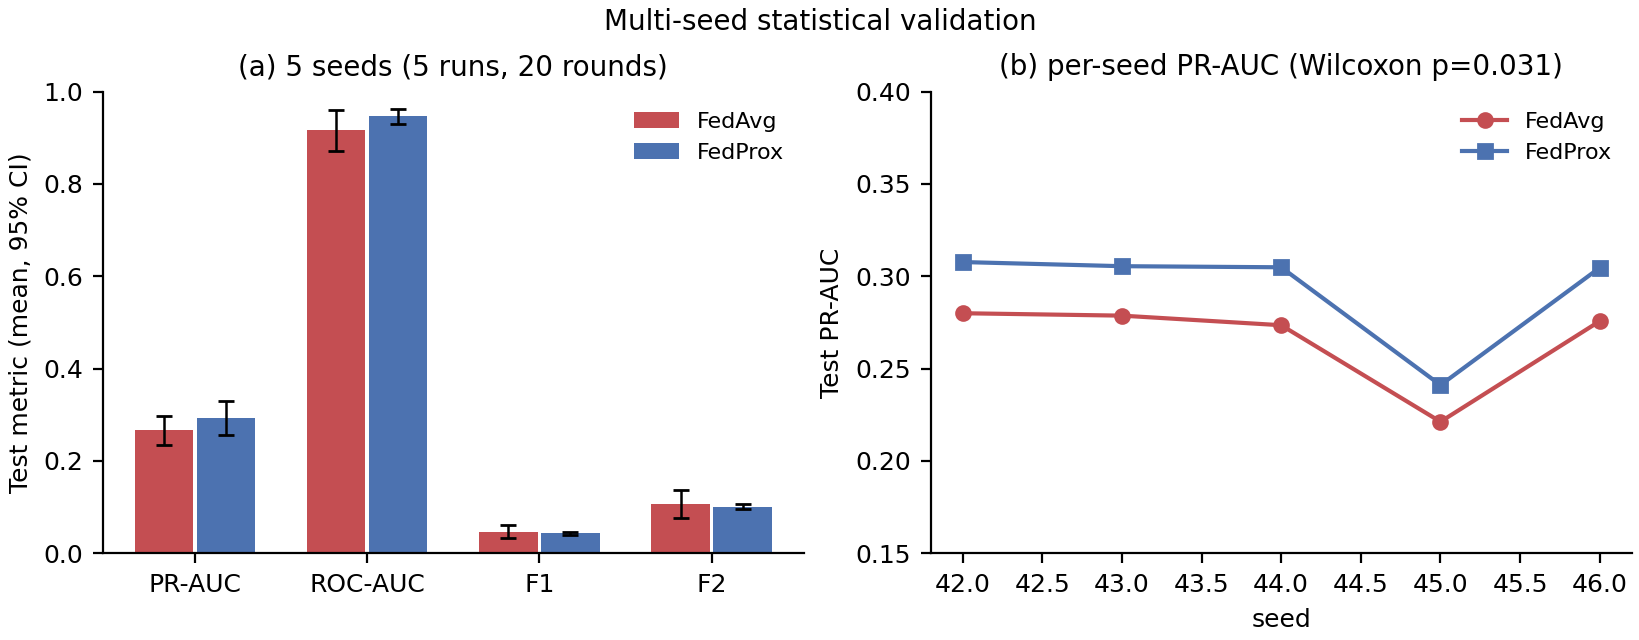
\includegraphics{figures/fig_multiseed.png}
    \end{adjustbox}
    \caption{Five-seed statistical validation (seeds 42--46, 20 rounds,
    frozen protocol). (a) Test metrics with 95\% confidence intervals.
    (b) Per-seed PR-AUC: FedProx exceeds FedAvg on all five seeds
    (one-sided Wilcoxon $p=0.031$).}
    \label{fig:multiseed}
\end{figure}

The v2.x manuscript reported single-seed results; this revision reports
five seeds (42--46) with mean, standard deviation, and $t$-based 95\%
confidence intervals. On the test set, FedProx achieves PR-AUC
$0.293 \pm 0.029$ (CI95 $\pm 0.036$) and ROC-AUC $0.946 \pm 0.013$
(CI95 $\pm 0.016$), against FedAvg's $0.266 \pm 0.025$ (CI95
$\pm 0.031$) and $0.916 \pm 0.036$ (CI95 $\pm 0.044$). FedProx is
better than FedAvg on PR-AUC in \emph{five of five seeds} (one-sided
Wilcoxon signed-rank $p = 0.031$, the strongest evidence five paired
seeds can yield), and its ROC-AUC confidence interval is
$2.7\times$ narrower. The $F_1$ difference is not significant
($p = 0.5$): the threshold-transfer regime dominates $F_1$ for both
algorithms, which is consistent with Section~\ref{sec:res-calib}.
What the five-seed study supports is a reproducibility claim about
the shipped pipeline: FedProx's superiority over FedAvg under the
frozen-protocol configuration is sign-consistent across every seed and
statistically significant. What it does not support is broad
generalisation, and---after Sections~\ref{sec:res-bn}
and~\ref{sec:res-nobn}---it must be read as a statement about the
composite (training $\times$ stale-buffer evaluation $\times$
saturated-monitor checkpointing), not about the algorithms in
isolation: every seed was evaluated through the same never-transported
BN statistics, and the no-BN control shows the underlying optimisation
gap is small. Five seeds is a small sample, the confidence intervals
quantify \emph{seed-to-seed variability} of this fixed configuration,
not the uncertainty of future observations or of other partitions, and
Section~\ref{sec:res-ablation} shows the shipped-eval gap narrows when
FedAvg is assisted by distribution-aware aggregation. The appropriate
summary is that FedProx was the most consistent stabiliser \emph{of the
shipped evaluation path} among the configurations studied, not that it
is load-bearing in every federated flare-prediction deployment.

\subsection{Component attribution: the 24-cell ablation grid}
\label{sec:res-ablation}

\begin{figure}[t]
    \centering
    \begin{adjustbox}{max width=\textwidth, max height=0.34\textheight}
        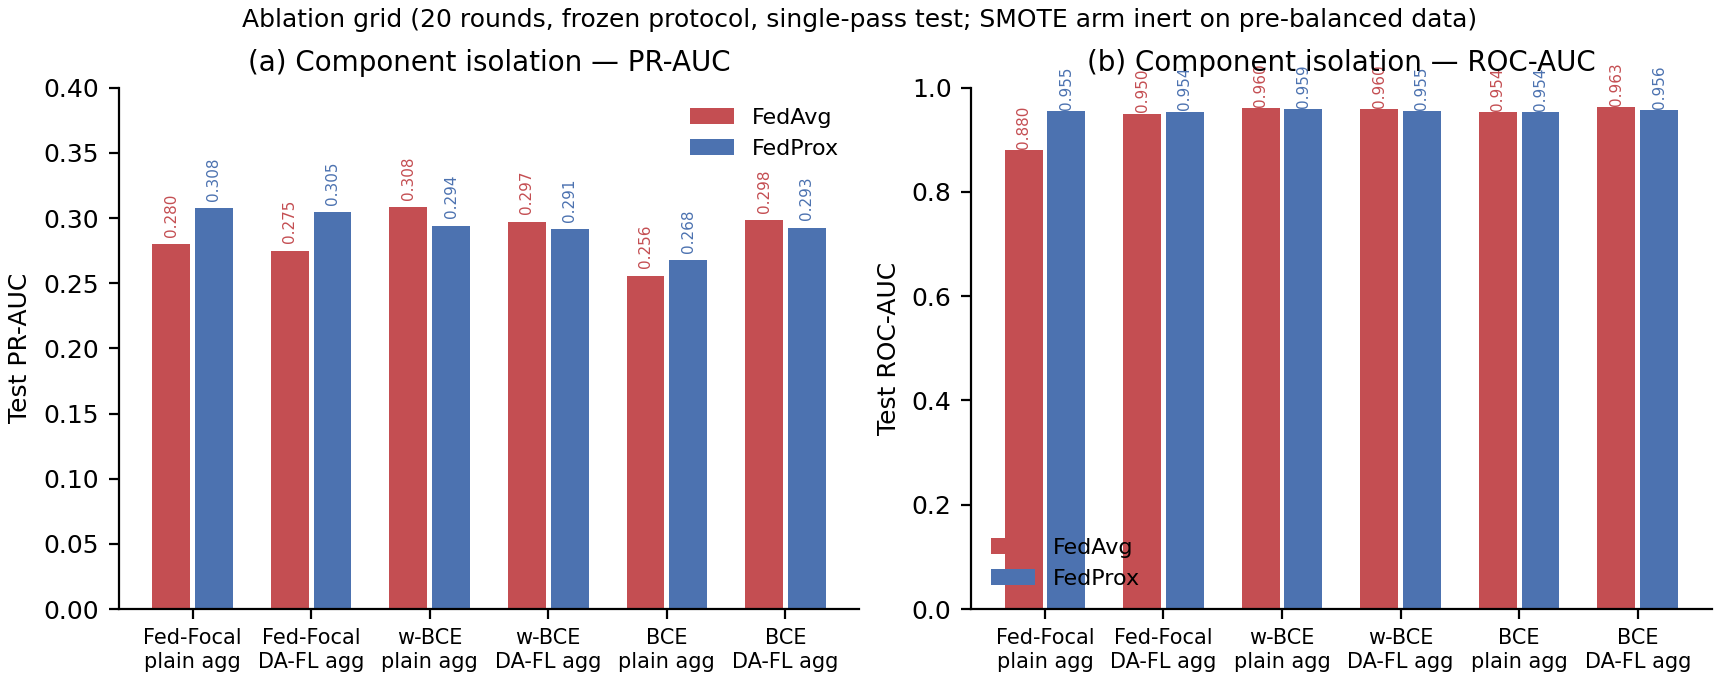
\includegraphics{figures/fig_ablation.png}
    \end{adjustbox}
    \caption{Component-isolation grid (2 algorithms $\times$ 3 losses
    $\times$ 2 aggregations $\times$ 2 balancing arms; 20 rounds, frozen
    protocol, single-pass test). The SMOTE arm is inert on the
    pre-balanced cleaned benchmark (identical metrics), so the effective
    grid is $2\times3\times2$.}
    \label{fig:ablation}
\end{figure}

Because the v2.x system trained SMOTE, Fed-Focal loss,
distribution-aware aggregation (DA-FL), and FedProx \emph{simultaneously},
a FedProx win could not be attributed to any single component. The
ablation grid isolates them (Fig.~\ref{fig:ablation}). Four patterns
emerge. \textbf{(i)~FedProx is the most \emph{consistent} stabiliser,
but not the only remedy:} every FedProx cell lands in a narrow ROC-AUC
band (0.954--0.959) whereas the FedAvg cells range from 0.880 (focal
loss, plain aggregation---the collapsing configuration) up to 0.963
(plain BCE with distribution-aware aggregation). That best FedAvg
cell \emph{exceeds} the FedProx headline (0.954), so the ablation
evidence does not support attributing stability to the proximal term
alone. \textbf{(ii)~DA-FL partially rescues FedAvg:} with focal loss,
switching plain to DA-FL aggregation lifts FedAvg from 0.880 to 0.950,
and the best cell overall (0.963) is plain BCE with DA-FL, suggesting
distribution-aware
weighting mitigates the same client-drift the proximal term
suppresses---at the cost of rate metadata sharing. \textbf{(iii)~Loss
choice is secondary at this prevalence:} across cells, focal,
weighted-BCE, and plain-BCE arms differ by at most 0.05 PR-AUC, with
weighted BCE marginally best for FedAvg-plain (0.308 vs 0.280).
\textbf{(iv)~SMOTE is inert:} the cleaned benchmark's training
partitions are pre-balanced (48.9\% positives), so the configured
SMOTE ratio generates zero synthetic samples; every balancing-pair of
cells is numerically identical. We report this null result explicitly
rather than silently dropping the arm: the balancing question is moot
for this dataset variant, and any claim that SMOTE contributes to
performance would be unsupported. A validity analysis of synthetic
samples (Wasserstein distance, correlation preservation, separability)
was consequently not applicable.

\subsection{Client-level heterogeneity: who benefits from federation?}
\label{sec:res-clients}

\begin{figure}[t]
    \centering
    \begin{adjustbox}{max width=0.96\textwidth, max height=0.34\textheight}
        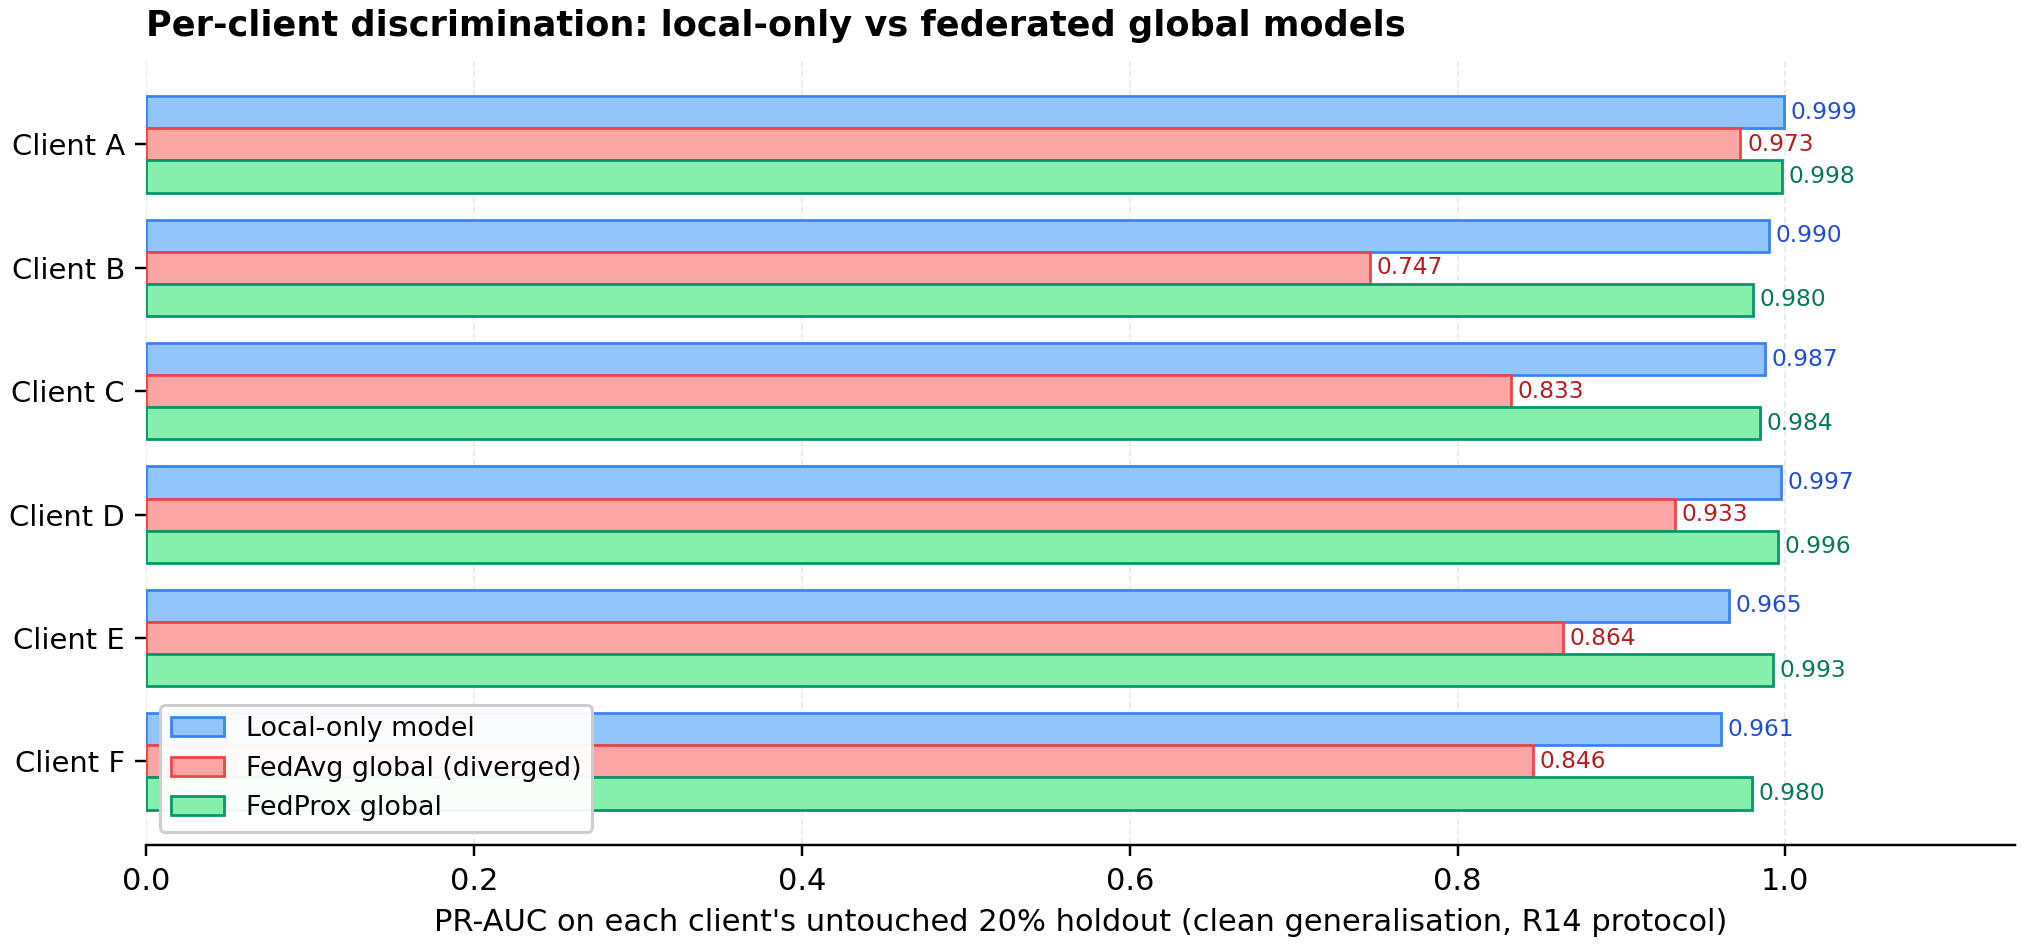
\includegraphics{figures/fig_clients.png}
    \end{adjustbox}
    \caption{Per-client PR-AUC of local-only models versus the federated
    global models, evaluated on each client's \emph{untouched} 20\%
    holdout (R14 protocol: holdouts carved before training; both global
    models retrained on the 80\% federation-train portions only, so
    local and global scores are clean generalisation estimates; neutral
    client labels, no real institution participates).}
    \label{fig:clients}
\end{figure}

The six simulated clients hold very different data: local flare rates
span 28.6\% (Client~B) to 80.5\% (Client~A), and
shard sizes span 1{,}503 (Client~E) to 23{,}418
(Client~B). Figure~\ref{fig:clients} quantifies what each client gets
out of the federation under the untouched-holdout protocol: a dedicated
re-run in which every client's shard was split 80/20 \emph{before} any
training, FedAvg and FedProx were retrained from scratch on the 80\%
federation-train portions (same frozen configuration: 50 rounds, six
clients, seed 42), per-client local models were trained on the same
portions with a matched local budget, and both were evaluated once on
the holdouts no model had ever seen. Three findings hold.
\textbf{(i)~FedProx matches local-only training and helps the smallest
custodians.} Mean PR-AUC is $0.988$ (FedProx global) versus $0.983$
(local-only); on the four largest clients the two are within
$0.001$--$0.010$ of each other, while the two smallest shards gain
clearly (Client~E: $0.965\to0.993$, $+0.027$; Client~F:
$0.961\to0.980$, $+0.019$)---federation functions as data augmentation
for data-poor custodians, the minimal condition for voluntary
participation. \textbf{(ii)~The diverged FedAvg average is worse for
everyone.} Its global model scores $0.747$--$0.973$ per client (mean
$0.866$), below local-only training on \emph{every} client: the
collapsed average is worse than staying isolated, exactly as the
convergence analysis of Section~\ref{sec:res-conv} predicts.
\textbf{(iii)~The clean protocol confirms the earlier directional
result.} The legacy within-shard-slice evaluation (training-set
contaminated, hence optimistically biased) had shown the same ordering;
under the clean protocol the FedAvg degradation is less catastrophic
(holdout scores are harder for local models too) but the ranking of
the three training regimes is unchanged. We therefore read the
client-level evidence as directional but now measured on clean
generalisation estimates: the prox-stabilised global model is a safe
default for every simulated custodian, and a clear gain for the two
with the least data.

\subsection{Interpretability across models}
\label{sec:res-shap}

\begin{figure}[t]
    \centering
    \begin{adjustbox}{max width=0.78\textwidth, max height=0.44\textheight}
        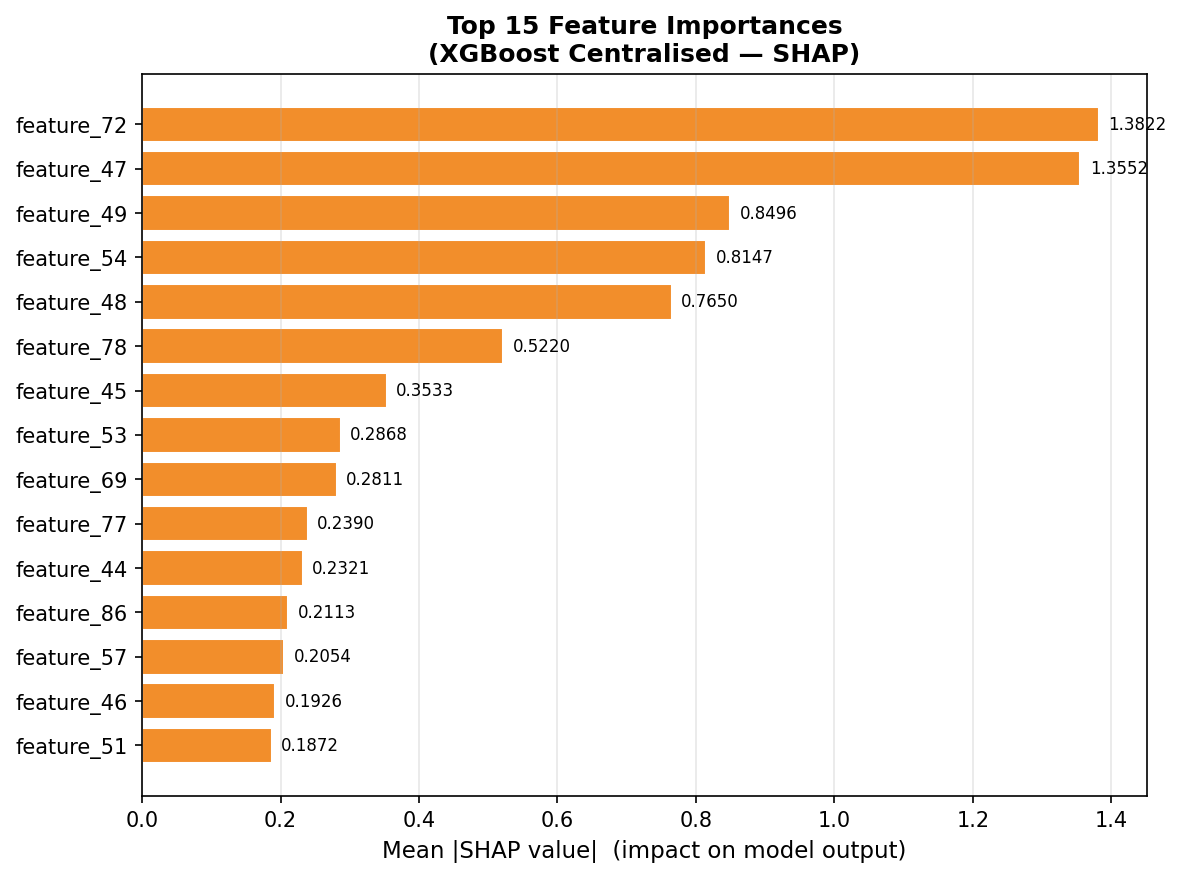
\includegraphics{figures/SHAP_Feature_Importance.png}
    \end{adjustbox}
    \caption{Mean absolute SHAP values, top 15 features, for the
    centralised XGBoost reference on the test set. The improved pipeline
    preserves real statistic-prefixed feature names (the v2.x pipeline
    reported generic indices, which this revision fixes).}
    \label{fig:shap}
\end{figure}

The v2.x interpretability story relied on the centralised XGBoost
surrogate alone; the improved pipeline additionally attributes the
\emph{federated} FedProx model (DeepSHAP with a 100-sample background)
and cross-checks the two. At the feature level the models agree only
moderately (Spearman $\rho = 0.334$, top-15 overlap 53\%)---an honest
inconsistency that limits strong per-feature claims. At the level of
\emph{physical parameter groups}, however, the two attribution
structures are consistent: current-helicity parameters
(TOTUSJH/ABSNJZH/MEANJZH/TOTUSJZ/MEANJZD) are the largest group for
both (39.9\% of XGBoost attribution mass, 29.0\% for FedProx), followed
by the R-value flux-emergence proxy (24.7\% / 23.2\%) and the Lorentz
force (22.7\% / 18.8\%). Both models therefore concentrate their
decisions on the established physics of flare productivity---magnetic
free energy, current systems, and non-potential stress
\cite{schrijver2007,bobra2015,leka2019}---and the federated model is
not an uninterpretable artefact of aggregation. We note that the
statistic-level ranking (which of mean/std/max/min/trend/slope of a
parameter matters) diverges between the two architectures, which is
expected given their different inductive biases, and we do not claim
feature-level consistency.

\subsection{Communication cost}
\label{sec:res-comm}

The global model has 29{,}377 parameters (0.117~MB at 32-bit
precision). Full-parameter exchange costs 117.5~KB per direction per
client per round: 0.235~MB round-trip, 1.41~MB per round across the
six-client cohort, and 70.5~MB aggregate over the 50-round run
(11.75~MB per client). These are \emph{parameter-exchange arithmetic}
from the frozen configuration---bytes counted, not measured on a live
deployment---and they quantify the \emph{training cadence} (one
round-trip per round) separately from the \emph{observation cadence}
(magnetogram records arrive every 12 minutes and the pooled windows
are spaced roughly 60 minutes apart; the global model
is refreshed per training cycle, while alerts can be emitted per
window). Wall-clock communication latency, aggregation compute,
client training time, straggler recovery, and secure-aggregation
bandwidth overhead were \emph{not} measured: the experiments ran
in-process on a single CPU container, with no real network. Enabling
secure aggregation would add a bounded multiplicative factor (mask
material per client per round), quantified in the deployment notes but
not evaluated here (Section~\ref{sec:threatmodel}).

\paragraph{Honest scaling against the data actually centralised.}
The relevant comparison is not raw magnetograms (our pipeline never
ships unprocessed data) but the feature arrays the centralised
alternative would need to receive once. On the cleaned substrate the
entire training feature set is $82{,}121 \times 144$ float32 values
(47.3~MB): the cohort's 50-round parameter exchange (70.5~MB) is
\emph{1.5 times larger}, so no bandwidth saving accrues for a single
training cycle at this model size --- communication frugality here is
a property of the continuous data stream (new records every
12 minutes) and repeated
retraining cycles, not of one run. On the raw 3D substrate the
ordering reverses: centralising the training windows
($214{,}888 \times 60 \times 24$ float32, $\approx$1.24~GB) exceeds
the LSTM cohort's lifetime parameter exchange at 32-bit round-trip
precision (219{,}265 parameters, $\approx$526~MB) by a factor of
2.4. The often-quoted $\approx$130~MB figure holds only under an
fp16 uplink-only convention that the code base lists as future
compression work, not as an implemented path; we state the
32-bit round-trip number as the honest default. Latency and
availability engineering remain deployment work.

\subsection{Data-locality cost analysis}

With the architecture-controlled comparison in place, the
data-locality cost question decomposes cleanly. Relative to the
\emph{same-architecture} centralised MLP, the federated model did not
underperform and in fact scored higher (ROC-AUC 0.954 vs 0.888; PR-AUC
0.307 vs 0.153) on this benchmark and configuration---an observation we
report with its two caveats: the federated arm consumed the larger
optimisation budget (Section~\ref{sec:budget}), and the mechanism is
consistent with a regularisation-like effect rather than a benefit of
federation as such. At this benchmark's scale, six disjoint shards with
29k parameters and a proximal regulariser behave like an
ensemble-like regulariser. Relative to the \emph{strongest available}
centralised reference (XGBoost, 300 trees), FedProx retains 97.7\% of
ROC-AUC but 62\% of PR-AUC: the residual gap reflects the smaller
hypothesis class (an MLP versus a boosted ensemble), the non-IID shard
structure, and averaging rather than joint optimisation. The honest
summary for a deployment decision: federation under this protocol cost
no ranking skill relative to a pooled MLP of the same class \emph{in
this study}; no raw magnetogram left any simulated client; and the
remaining gap to the tree-ensemble reference is an architecture-budget
question, not a data-locality question. What the study does \emph{not}
establish is that these in-partition numbers generalise: budget
parity and natural-prevalence retraining have both since been
executed (the gap survives budget parity, Section~\ref{sec:budget},
but is substrate- and encoder-conditional,
Section~\ref{sec:res-raw}), and within-fold region-disjoint
validation remains the open item (Section~\ref{sec:limitations}).
